\subsection{Discovery}\label{subsec:wotdiscovery}

Die \glsxtrshort{wt}-Discovery beschreibt einen Prozess, mit dem eine \glsxtrfull{td} gefunden werden kann.
Dabei soll die Verbreitung in einer Vielzahl von Anwendungsfällen unterstützen werden, wie Beispielsweise in lokalen und öffentlichen Netzwerken.
Der Prozess muss dabei mit bestehenden Discovery-Mechanismen funktionieren, sicher sein und private Informationen schützen.
Es muss ebenfalls in der Lage sein, Aktualisierungen von \glspl{td} effizient zu handhaben.

\begin{figure}[H]
    \centering
    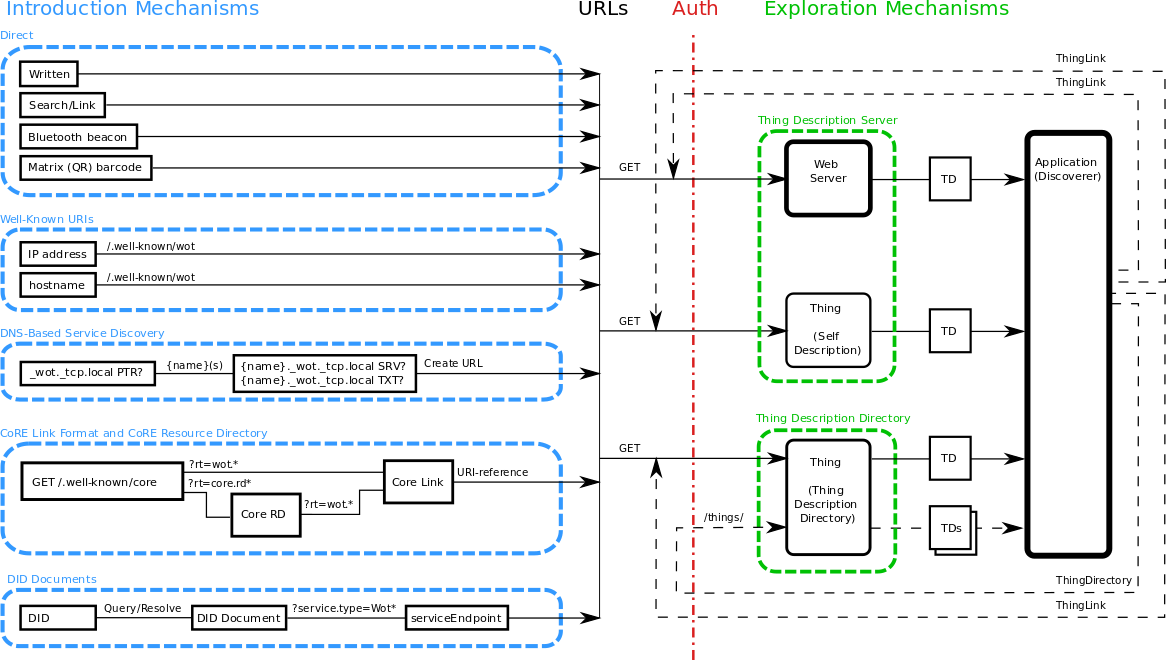
\includegraphics[width=16cm]{discovery-overview.png}
    \caption{Discovery-Architektur}\label{fig:discovery_overview}
\end{figure}

Der \gls{sd} Prozess ist dabei in zwei Phasen unterteilt, die Einführungs- und die Erkundungsphase.
Die Einführungsphase nutzt bestehende Erkundungsmechanismen, um ein oder mehrere \glspl{url} zu erzeugen.
Diese \glspl{url} enthalten selbst keine Metadaten und verweisen auf Erkundungsdienste.
Erst diese Erkundungsdienste stellen dann Metadaten in Form von \gls{td}[s] und \glspl{tdd} bereit.
Dabei gibt es zwei Arten von Erkundungsdiensten:

\begin{itemize}
    \item Ein Dienst, der sich um die Verteilung einer einzelnen \gls{td} kümmert, wie z.\,B.\ ein einfacher Webservice.
    \item Ein Dienst für das Durchsuchen eines \gls{tdd}[s], worin sich mehrere \gls{td}[s] befinden.
\end{itemize}

Der Discovery-Prozess verwendet eine zweistufige Architektur.
Im ersten Schritt generieren die Einführungsmechanismen \glspl{url}, die dann in der Erkundungsphase referenziert und mit Metadaten verknüpft werden.
Die Einführung kann durch jeden Mechanismus durchgeführt werden, der eine \gls{url} liefern kann.
Der Einführungsmechanismus kann dabei auch mehrere \glspl{url} liefern, die in der Erkundungsphase in mehreren \glspl{td} resultiert.
Eine \gls{url}, die von einem Einführungsmechanismus zur Verfügung gestellt wird, zeigt dabei immer auf einen Endpunkt eines Erkundungsmechanismus, der eine \gls{td} liefert.
Dies ist im einfachsten fall eine gewöhnliche Ressource, die von einem Webserver bereitgestellt wird und eine \gls{td} zurückgibt.
Im Sonderfall gibt es noch eine selbst beschreibende \gls{url} für ein \gls{thing}, was seine eigene \gls{td} liefert.

Jeder Client, der eine einzelne \gls{td} mit einer einzelnen \gls{url} abrufen kann, unterstützt \glsxtrshort{wot}-Discovery.
Sie muss dabei aber gewisse Anforderungen erfüllen, wie z.\,B.\ dass mindestens ein Einführungsmechanismus vorhanden sein muss
oder das mehrere Aufrufe desselben Einführungsmechanismus möglich sind.
Diese Anforderungen sorgen dafür, dass genau definiert ist, wie sich die \gls{td} in verschiedenen Szenarien verhalten soll.
Es können verschiedene Einführungsmechanismen verwendet werden, wie z.\,B.\ die direkte Variante über eine \gls{url}, eine Variante mit DNS-basierter Service-Discovery, oder eine Variante mithilfe von \gls{core}.
Das Ergebnis ist aber immer eine \gls{url} eines Erkundungsmechanismus, welcher die Metadaten einer \gls{td} beinhaltet.

Im Erkundungsprozess werden \glspl{td} mithilfe von zwei Mechanismen über einen Server zur Verfügung gestellt.
Jeder Webdienst, der über eine \gls{url} referenziert werden kann und eine \gls{td} zurückliefert, kann als Erkundungsmechanismus verwendet werden und wird als \glsxtrshort{td}-Server bezeichnet.
Ein \glsxtrshort{td}-Server muss dabei nicht zwangsläufig ein \gls{thing} sein, sondern kann auch über ein einfachen Webserver implementiert werden.
\glsxtrshort{td}-Server können auch zur Selbstbeschreibung verwendet werden. Für die Selbstbeschreibung hostet ein \gls{thing} seine eigene \gls{td} und stellt sie zur Verfügung.
Neben \glsxtrshort{td}-Servern gib es noch die bereits erwähnten \glspl{tdd}, worin sich keine oder mehrere \gls{td}[s] befinden und verwaltet werden können.
Für jede \gls{td} enthält das \gls{tdd} zusätzliche Metadaten für Buchführungs- und Suchzwecke.
